\section{Simulation experiments}
\label{sec:simulation}
In this section, we study the usefulness of coordinating information gathering activities in a target tracking domain.
To the best of our knowledge, there are currently no methods directly comparable to ours that address the same problem.
The related approaches~\cite{Nair2005,Renoux2015} require transition and observation independence, and the auctioning method proposed in~\cite{Capitan2013} and the multi-robot Dec-POMDP studies~\cite{Omidshafiei2015,Omidshafiei2016} use state and action based rewards.
Instead, we compare optimal $\rho$Dec-POMDP policies to hand-tuned heuristic policies.

\subsection{Cooperative target tracking domain} 
In the scenario of Figure~\ref{fig:example}, the state consists of the target location $l \in \{l_1, l_2, l_3, l_4\} = L$ and a binary variable describing the target status; neutral (0) or hostile (1).
The target does not change its status, but moves in a different pattern depending on the status.
A neutral target stays in place with probability $p_0$, and moves to either neighbouring location with probability $(1-p_0)/2$.
A hostile target stays in place with probability $p_1$.
We set $p_0 = 0.85$ and $p_1 = 0.6$.

Both MAVs have two actions, $a_c$ and $a_r$, referring to applying a camera or a radar, respectively.
The observations $\Z_1=\Z_2=L$ correspond to perceiving the target at any of the locations.
The observations do not provide information on the target status, which has to be inferred based on a series of observations.
Sensor accuracy depends on the distance to the target.
At $l_1$, the target is at distance 0 from MAV 1, and at distance 3 from MAV 2, at $l_2$, the distances are 1 and 2, and so on.
We model the sensors by Gaussian distributions with mean at the target location, and standard deviation dependent on the target status and increasing as a function of the distance.
For a sensor mode $j$, given a distance $d$, its standard deviation is $\sigma_j(d) = \sigma_{j,0} \cdot 2^{(d/d_{j,0})}$, where $\sigma_{j,0}$ is the nominal standard deviation, and $d_{j,0}$ is the half efficiency distance of the sensor.
The parameters we applied are summarized in Table~\ref{tab:obsmodel}.

\begin{table}[]
\centering
\caption{Sensor parameters in the simulation.}
\label{tab:obsmodel}
\begin{tabular}{@{}ccccc@{}}
\toprule
            & \multicolumn{2}{c}{Neutral target} & \multicolumn{2}{c}{Hostile target} \\ \midrule
Sensor mode $j$ & $d_{j,0}$      & $\sigma_{j,0}$  & $d_{j,0}$       & $\sigma_{j,0}$            \\ \midrule
camera              &   0.6      &  0.3            &   0.7           & 0.75             \\
radar               &  1.0       &  0.2            &   1.0           & 0.45             \\
radar (interference)&  2.0       &  1.0            &   1.5           & 1.2             \\ \bottomrule
\end{tabular}
\end{table}


The reward is as in Eq.~\eqref{eq:rhoreward}, with $\alpha = 1$ and $g$ as Shannon entropy.
In $R(s,a)$, for each agent applying the radar action $a_r$, there is a reward of -0.1, and additionally, if the target is hostile, an additional reward of -1 or -0.1 if the target is at distance 0 or 1, respectively.
This term models the higher costs of applying the radar, and the risk of revealing the MAVs' own location to a hostile target if radar is engaged at short range.

\subsection{Experimental results}
We varied the communication interval $c$ and the initial joint belief state $b_0$.
We compare the value of an optimal policy of the $\rho$Dec-POMDP\footnote{We apply MAA* from the MADP toolbox \url{www.fransoliehoek.net/madp/}, extended by us to handle information theoretic rewards.} to five heuristic policies.
Policy 1 is a risk-averse strategy where both MAVs only apply cameras.
In policy 2, the first MAV always applies its camera, and the second MAV always applies its radar.
Policy 3 is the same as policy 2, reversing the roles.
Policy 4 is a turn-taking policy where the first MAV starts by applying its camera while the second MAV applies its radar, and on subsequent time steps they switch sensors; policy 5 is the same with reversed roles.

We set $b_0$ uniform with respect to the target's location, and varied the initial probability that the target is neutral.
Figure~\ref{fig:pfriendly} shows the values of the policies for $h=3$ as function of the probability that the target is neutral.
If it is very likely that the target is hostile, the heuristic policy of only applying the cameras is close to optimal as it avoids the risk of additional costs for radar use on hostile targets.
The cameras only policy has a much lower value when it is more likely that the target is neutral.
In this case, the other heuristic policies all work equally well, and are close to optimal.
None of the heuristic policies can consistently reach near-optimal performance.
An important advantage of an optimal policy is that it adapts to changing situations, unlike the fixed heuristic policies.

\begin{figure}[t]
\centering
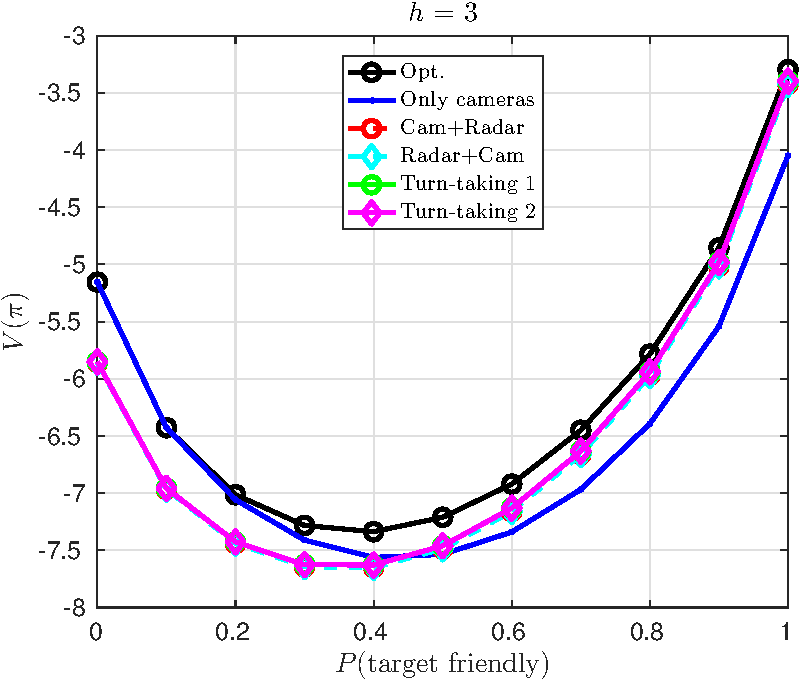
\includegraphics[width=0.8\columnwidth]{fig/target_friendly.pdf}
\caption{Values of optimal and heuristic policies as a function of the initial probability of the target being neutral. The policies corresponding to the red, cyan, green and magenta lines have almost equal values and overlap each other.}
\label{fig:pfriendly}
\end{figure}

We then set $b_0$ uniform, and varied the communication interval $c$ between 1 and 3.
At every $c$th time step, a new policy for horizon $h=3$ was computed and then applied for the next $c$ decisions.
We ran 50 simulations on the task, each for 51 decisions, recording the rewards for each policy.
Table~\ref{tab:rewards} shows the average total rewards with 95\% confidence intervals for an optimal policy for $h=3$ while varying $c$, each heuristic policy, and a policy of choosing random actions.
Policies 2 and 3 are grouped together as ``fixed roles'', and 4 and 5 as ``turn-taking'' as there was no significant difference between them.
Here the optimal policy performs equally well regardless of the communication interval, while the turn-taking policy also performs well.
The lack of improvement for lower $c$ is explained by the fact that the actual horizon of the task is equal to 51, the number of decisions to be taken, which is much longer than the planning horizon applied.

\begin{table}[]
\centering
\caption{Average rewards with 95\% confidence intervals.}
\label{tab:rewards}
\begin{tabular}{@{}ccc@{}}
\toprule
Policy             & Comm. interval & Reward \\ \midrule
\multirow{3}{*}{Optimal} & 1  &  -89.9 $\pm$ 1.2    \\
                   & 2  & -90.1 $\pm$ 1.6   \\
                   & 3  &  -89.8 $\pm$ 1.2    \\ \midrule
Cameras only        & - &  -96.6 $\pm$ 2.0    \\
Fixed roles        & - &  -95.0 $\pm$ 1.5   \\
Turn-taking        & - &  -90.7 $\pm$ 1.4   \\
Random             & - &  -104.2 $\pm$ 2.1   \\ \bottomrule
\end{tabular}
\end{table}

